\ifdefined\standalone 
\documentclass[12pt]{article}
\usepackage{graphicx}
\usepackage{float}
\usepackage[a4paper, margin=1in]{geometry}
\usepackage[utf8]{inputenc}
\usepackage{textcomp}
\usepackage{amsmath}
\usepackage{booktabs}
\usepackage{tikz}
\usepackage{enumitem}
\usetikzlibrary{decorations.pathmorphing,patterns}
\usepackage[hidelinks]{hyperref} % <- hypertext

\begin{document}
\fi

\section{Mixed heat transfer}
This verification case assesses the capability of Gpyro to accurately represent 1D heat transfer involving multiple modes of transfer, and compares the results with those from FDS. The scenario consists of a medium-density fibreboard (MDF) sample subjected to a cone calorimeter test in a nitrogen atmosphere. The properties of the simulated materials can be found in table \ref{tab:phys_props_mdf}. The material is exposed to an external heat flux of $q''_{ext}=1~\mathrm{kW/m^2}$ and ambient air at 25~$^\circ$C, with a convection coefficient of $h_c = 10~\mathrm{W\,m^{-2}\,K^{-1}}$.

\begin{table}[H]
\centering
\caption{Thermophysical properties of MDF}
\label{tab:phys_props_mdf}
\renewcommand{\arraystretch}{1.3} % spacing between rows
\begin{tabular}{c c c c}
\hline
$k$ ($\mathrm{W\,m^{-1}\,K^{-1}}$) & 
$c_p$ ($\mathrm{J\,kg^{-1}\,K^{-1}}$) & 
$\rho$ ($\mathrm{kg\,m^{-3}}$) & 
$\varepsilon (-)$ \\
\hline
0.15 & 1340 & 605 & 0.86 \\
\hline
\end{tabular}
\end{table}

The results obtained using Gpyro are compared to those from FDS. Figure~\ref{fig:mixed_temp} presents the comparison of the temperature evolution in time at various depths.
\begin{figure}[H]
\centering

\begin{minipage}[t]{0.45\textwidth}
\centering
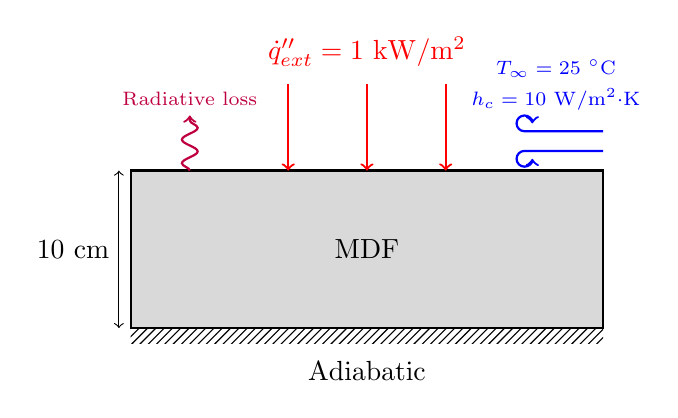
\begin{tikzpicture}[scale=1.0]
% MDF block
\draw[fill=gray!30,thick] (0,0) rectangle (6,2); 
\node at (3,1) {MDF};

% Adiabatic bottom
\fill[pattern=north east lines] (0,-0.2) rectangle (6,0);
\node[below] at (3,-0.3) {Adiabatic};

% Dimension line for height
\draw[<->] (-0.15,0) -- (-0.15,2);
\node[left] at (-0.15,1) {10~cm};

\foreach \x in {1.8,2.8,3.8}
    \draw[->,thick,red] (\x+0.2,3.1) -- (\x+0.2,2);

\node[above,red] at (3,3.2) {$\dot{q}''_{ext} = 1~\mathrm{kW/m^2}$};

\draw[->,thick, blue] (6,2.25) -- (5,2.25) arc[start angle=90, end angle=360, radius=0.1cm]; 
\draw[->,thick, blue] (6,2.5) -- (5,2.5) arc[start angle=270, end angle=0, radius=0.1cm]; 

\node[blue] at (5.4,2.9) {\scriptsize $h_c = 10~\mathrm{W/m^2{\cdot}K}$};
\node[blue] at (5.4,3.3) {\scriptsize $T_\infty = 25~^\circ\mathrm{C}$};

\draw[purple,thick,->,decorate,decoration={snake,amplitude=1mm,segment length=3mm}] (0.75,2) -- (0.75,2.7);

\node[above,purple] at (0.75,2.7) {\scriptsize Radiative loss};
\end{tikzpicture}
\caption{Configuration schematic}
\label{fig:mixed_configuration}
\end{minipage}
\hfill
\begin{minipage}[t]{0.45\textwidth}
\centering
\includegraphics[width=\linewidth]{conv_rad.png}
\caption{Temperature evolution comparison}
\label{fig:mixed_temp}
\end{minipage}
\end{figure}

\ifdefined\standalone
\end{document}
\fi






